\subsection{Descripci\'on del problema}

\noindent
Se pide resolver la problem\'atica que tiene una empresa transportadora en reducir \'optimamente la cantidad de camiones que utiliza para transportar una serie de productos qu\'imicos. \\
Dada una cierta cantidad n de productos qu\'imicos, tal que para cada par de combinaciones de productos se corresponde un valor num\'erico mayor o igual a 0 llamado coeficiente de peligrosidad (un coeficiente por cada par), debemos reducir al m\'inimo la cantidad de camiones que utilizamos para transportar los n productos siendo que existe un valor M, num\'erico mayor o igual a 0, que llamaremos umbral de peligrosidad, y cuyo valor debe ser mayor o igual a la suma de todas las peligrosidades dentro de un cami\'on. La suma de todas las peligrosidades dentro de un camion, como esta expresado, es lo mismo que la suma de todos los coeficientes de peligrosidad de todas las combinaciones de pares de productos que se encuentren en el cami\'on. 
\bigskip

\noindent
Ejemplo1: \\
$n = 2$ y $M = 0$ \\ 
$peligrosidad_{(0,1)} = 1$ \\
(la peligrosidad de los dos quimicos juntos es de 1) \\

\noindent
La cantidad m\'inima de camiones necesarios para transportar los qu\'imicos es 2. La raz\'on es que la peligrosidad de la combinaci\'on de los dos qu\'imicos es 1. Luego si la peligrosidad de un camion es la suma de todas sus peligrosidades por combinaciones de qu\'imicos y contiene a los qu\'imicos 0 y 1, la peligrosidad del cami\'on es 1. Y 1 es mayor a M, por lo tanto poner estos dos quimicos en el mismo cami\'on no es una opci\'on. \\
La \'unica opci\'on de poner los dos quimicos separados, osea en distintos camiones. Como s\'olo teniamos 2 qu\'imicos y ambos est\'an en alg\'un cami\'on, esta es la soluci\'on. 
\bigskip
\bigskip

\noindent
Ejemplo2: \\
$n = 3$ y $M = 1$ \\
$peligrosidad_{(1,2)} = 2$ \\
$peligrosidad_{(0,1)} = 0$ \\
$peligrosidad_{(0,2)} = 0$ \\

\noindent
En este caso la cantidad m\'inima de camiones es 2. \\
Se tiene que la \'unica combinaci\'on de quimicos que agrega peligrosidad a un cami\'on es la de los qu\'imicos 1 y 2. Estos dos qu\'imicos no pueden estar juntos, deben estar separados en 2 camiones distintos ya que su combinaci\'on supera a la cota de peligrosidad M. Establecemos entonces que debemos tener desde ya dos camiones, uno para el qu\'imico 1 y otro para el 2. 
Analizando el qu\'imico 0 podemos ver que no importa con qu\'e qu\'imico este combinado, no agrega peligrosidad a un cami\'on. Puede ser ubicado en cualquiera de los dos camiones, no hace falta agregar otro cami\'on para ubicar este qu\'imico.
\bigskip
\bigskip

\noindent
Ejemplo3: \\
$n = 3$ y $M = 50$ \\
$peligrosidad_{(1,2)} = 1$ \\
$peligrosidad_{(0,1)} = 2$ \\ 
$peligrosidad_{(0,2)} = 1$ \\ 

\noindent
En este caso la cantidad m\'inima de camiones es 1. Ya que la peligrosidad de poner los 3 qu\'imicos en un mismo cami\'on es la peligrosidad de (1,2) + (0,1) + (0,2) = 1 + 2 + 1 = 4 < M (=50). Y dado que no hay soluci\'on m\'as chica que poner todos los qu\'imicos en 1 s\'olo cami\'on, \'esta es la mejor soluci\'on.
 
\subsection{Resoluci\'on}

\noindent
Para resolver el problema utilizamos la t\'ecnica de backtracking. \\
Comenzamos creando un primer cami\'on y ubicando un qu\'imico en \'el. Luego llamamos a la funci\'on recursiva descripta a continuaci\'on. \\
La funci\'on recursiva hace lo siguiente: \\
Se fija si todos los qu\'imicos estan ubicados en alg\'un cami\'on, \\
1- De ser verdadero resulta que nos encontramos con una soluci\'on posible al problema. Se testea que esta posible soluci\'on sea mejor a una soluci\'on previamente guardada (ser mejor en este caso significa que tenga menor n\'umero de camiones). Si es efectivamente mejor o no hab\'ia soluci\'on guardada (es el caso de la primera vez que pasa por ac\'a, se guarda la soluci\'on nueva pisando a la guardada si lo hubiese. \\
2- De ser falso, resulta que quedan quimicos por ubicar. Entonces lo que hace es iterar sobre todos los qu\'imicos no ubicados en alg\'un cami\'on y por cada quimico iterar sobre los camiones ya creados y 1 camion nuevo sin quimicos. En cada cada iteracion se prueba si la peligrosidad resultado de ubicar el quimico en el camion es menor o igual a la cota M. De ser as\'i se coloca el quimico en el camion y se llama nuevamente a la funcion recursiva. Cuando se vuelve de la funcion recursiva se quita el quimico del camion y se continua con la proxima iteraci\'on. \\
Una vez se recorran todas distribuciones posibles, la soluci\'on al problema se encuentra en aquella que est\'e guardada, mencionada anteriormente. \\
\noindent
En la implementaci\'on del algoritmo identificamos a los qu\'imicos por un identificador numerico \'unico. Cada qu\'imico toma ese n\'umero sobre el rango [0..n]. 

\bigskip
\bigskip
\noindent
$\proc{BIOHAZARD(M):}$
\begin{itemize}
	\item Creo el primer cami\'on.
	\item Agrego el qu\'imico con identificador 0 al primer cami\'on.
	\item RECURSION(infoCamiones(*), 1, n)		
\end{itemize} 
\bigskip
\bigskip

\noindent
$\proc{RECURSION(infoCamiones, q(**), M)}$
\begin{itemize}
	\item Si est\'an todos los qu\'imicos cargados en alg\'un cami\'on,							
	\begin{itemize}
		\item El estado actual de los qu\'imicos (d\'onde est\'an ubicados) es una posible soluci\'on
		\item Si la cant. de camiones que se est\'an usando en esta posible soluci\'on es menor a la m\'as chica que encontr\'e,
		\begin{itemize}
			\item Guardo esta posible soluci\'on c\'omo la que tiene menos camiones entre todas las ya encontradas.
		\end{itemize}																												
		\item Sino,
		\begin{itemize}
			\item Por cada cami\'on que ya contenga al menos 1 qu\'imico,									
			\begin{itemize}
				\item Si la peligrosidad de agregar el qu\'imico $q$ en \'este cami\'on no supera a $M,$
				\begin{itemize}
					\item Agrego el qu\'imico $q$ a este cami\'on
					\item $\proc{RECURSION(q++, M)}$
					\item Quito el qu\'imico $q$ de este cami\'on
				\end{itemize}
			\end{itemize}		
		\end{itemize}
		\item Si la poda 2 no est\'a habilitada, o si agregar un cami\'on no hace que la cantidad de camiones sea igual o mayor a la de la soluci\'on guardada, (si la hay, de lo contrario tambi\'en prosigo),
		\begin{itemize}
			\item Creo un nuevo cami\'on.
			\item Agrego el qu\'imico $q$ al nuevo cami\'on.
			\item $\proc{RECURSION(infoCamiones, q++, M)}$	
			\item Quito el qu\'imico $q$ del nuevo cami\'on.
			\item Elimino el nuevo cami\'on.
		\end{itemize}
	\end{itemize}			
\end{itemize}
\bigskip
\noindent
(*): infoCamiones contiene la informaci\'on de cuantos camiones hay creados, cuantos y cuales qu\'imicos contiene y cual es el valor de la peligrosidad del cami\'on con los qu\'imicos que tiene actualmente. En la implementaci\'on, esta informaci\'on en realidad se guardan sobre otras estructuras, pero para fines te\'oricos lo definimos ac\'a de esta manera.\\
(**): $Q$ es el identificador de un qu\'imico.
\bigskip
\bigskip

\noindent
Implementamos podas para ayudar mejorar los tiempos de ejecuci\'on. Las podas son 2. 

\noindent
La primera poda es no permitir soluciones \textbf{practicamente iguales}. Donde una solucion es practicamente igual a otra si tiene los mismos conjuntos de quimicos ubicados por cami\'on pero est\'an ubicados en diferentes numero de camion. Por ejemplo las siguientes podr\'ian ser dos soluciones \textbf{practicamente iguales}:
$2 0 0 1 1$
$2 1 1 0 0$
 
\noindent
La segunda poda es no recorrer ramas tal que pueda deducir que sus hojas y posibles solucion no puedan mejorar la que ya esta guardada como mejor hasta el momento. Por ejemplo si encontr\'e una posible soluci\'on que utiliza s\'olo 2 camiones, y me encuentro recorriendo una rama que lleva por el momento 3 camiones con qu\'imicos faltando qu\'imicos por ubicar. Esta intuici\'on va a ser explicada con m\'as detalle m\'as adelante.


\subsection{Correctitud}

\noindent
Justificaci\'on de podas.

\noindent
Primera poda: 
Como dijimos la soluci\'on de esta poda se encuentra en los numeros de identificadores de los qu\'imicos y qu\'e numero de identificador se le da a un cami\'on recientemente creado.\\
Cada qu\'imico tiene un numero de identificador distinto que va desde 0 hasta n-1. En las iteraciones se itera por cada qu\'imico no ubicado, desde el de menor numero de identificador hasta el mayor.\\ 
Cada cami\'on nuevo tiene un n\'umero de identificador de +1 al \'ultimo creado. \\
El efecto de resolverlo de \'esta manera es que si un qu\'imico se ubica en un cami\'on nuevo, s\'olo los qu\'imicos de n\'umero de identificador mayor se pueden ubicar en el mismo grupo. Y si por cada cami\'on nuevo su n\'umero de identificador es mayor, el efecto es el siguiente:\\
Cada qu\'imico $q$ est\'a ubicado en el n\'umero de cami\'on $X$, tal que el n\'umero de qu\'imico m\'as chico del grupo del qu\'imico $q$ es el numero $X$ en la lista ordenada de menor a mayor de los menores identificadores de qu\'imicos de cada grupo. Dado que todos los qu\'imicos tienen un n\'umero de identificador distinto \'existe una univoca soluci\'on que cumpla estas caracteristicas, no hay soluciones practicamente iguales.\\

\noindent
Segunda poda:
Definimos un $estado$ en el contexto de nuestro algoritmo como cierta configuracion de qu\'imicos tal que ciertos o ning\'un qu\'imico est\'an ubicados en determinados camiones, y ciertos otros o ning\'un qu\'imico no estan ubicados en ning\'un cami\'on.
Definimos una soluci\'on incompleta como un estado donde hay 1 o m\'as qu\'imicos no ubicados en camiones. \\
Una soluci\'on incompleta es el padre de una rama del arbol de estados posibles generado por el algoritmo. Todos la descendencia de la soluci\'on incompleta, son todas las configuraciones que mantengan los mismos qu\'imicos ubicados en los mismos camiones mientras que var\'ien los qu\'imicos que no est\'aban ubicados en ning\'un cami\'on.
Dada cualquier solucion incompleta, la cantidad de camiones de su descendencia no puede hacerse m\'as chica. Esto se debe a que, como aclaramos antes, la descendencia debe mantener la configuraci\'on de qu\'imicos y camiones de su ascendencia, y por lo tanto no puede eliminar camiones de que ten\'ia su ascendencia. \\
Debido a esto, podemos garantizar que si el estado del padre de una rama tiene una cantidad de camiones mayor o igual a la de una soluci\'on ya previamente guardada. Su descendencia tambi\'en va a tener por lo menos una cantidad de camiones mayor o igual a la soluci\'on guardada. Y dado que se busca una soluci\'on tal que sea la que menos camiones tenga, s\'olo nececito buscar siempre soluciones mejores a las encontradas, no iguales ni peores.\\
Esto lleva a que, una vez detectada las soluciones no mejores, estas se desechen antes de que generen descendencia.\\


\subsection{Complejidad del algoritmo}


\noindent
Debemos aclarar en primer lugar que el algoritmo de backtracking genera un arbol de posibilidades con una rama nueva por cada llamada a la funci\'on recursiva. En particular, en nuestro algoritmo cada nodo lo identificamos como una configuraci\'on de qu\'imicos en camiones especificos. A su vez tambi\'en es el c\'odigo que se ejecuta para llegar de una configuraci\'on de quimicos a otra.

\noindent
Cierto c\'odigo \textbf{combinar2} se ejecuta una vez por cada nodo en el arbol y var\'ia dependiendo del estado anterior. \\
En particular cada nodo comienza ejecutando el siguiente codigo:

\lstset{language=C++,
                basicstyle=\ttfamily\footnotesize,
                keywordstyle=\color{blue}\ttfamily,
                stringstyle=\color{red}\ttfamily,
                commentstyle=\color{green}\ttfamily,
                morecomment=[l][\color{magenta}]{\#},
                breaklines=true
}
\begin{lstlisting}

if (quimicoACargar == this->n) {
	if (minCamiones > camiones.size()){                                 
		if (this->mostrarInfo) mostrarSolucion(carga, camiones.size());
		this->minCamiones = camiones.size();
		this->cargaMinima = carga;
	}
	return;
}
%\end{lstlisting}

\noindent 
$quimicoACargar == this->n$ corresponde a consultar si el nodo es soluci\'on. O, lo que es lo mismo, si es hoja. Comparacion de enteros la despreciamos \textbf{O(1)}.\\
De ser hoja se fija si la soluci\'on encontrada es mejor a una anterior encontrada, comparaci\'on de enteros \textbf{O(1)}. Podemos suponer el peor caso, que esto sea cierto. Luego cambia la soluci\'on guardada por la soluci\'on actual. Esto tiene un costo de copiar un vector<int> de tamanio $n$, es decir \textbf{O(n)}.\\
Finalmente deducimos que todo este c\'odigo tiene un costo de \textbf{O(n)} para las hojas y de \textbf{O(1)} para el resto de los nodos.

\noindent 
La segunda cuota de codigo es la siguiente:

\begin{lstlisting}

list<Camion>::iterator itCamion;
for (itCamion = camiones.begin(); itCamion != camiones.end(); itCamion++){
	int peligrosidadAgregada = 
      calcularPeligrosidadAgregada(*itCamion, quimicoACargar);    
	if (this->M >= (itCamion->peligrosidad + peligrosidadAgregada)){                  
			itCamion->quimicos.push_back(quimicoACargar); O(1)
		itCamion->peligrosidad += peligrosidadAgregada;   O(1)
		carga[quimicoACargar] = itCamion->nro;            O(1)
		combinar2(camiones, quimicoACargar+1, carga);     O(f)
		carga[quimicoACargar] = -1;                       O(1)
		itCamion->peligrosidad -= peligrosidadAgregada;   O(1)
		itCamion->quimicos.pop_back();                    O(1)
	}
}
\end{lstlisting}

\noindent 
Identificamos varias operaciones simples de asignaci\'on y comparaci\'on de enteros y un push y pop en una lista de enteros, todas despreciaremos a \textbf{O(1)}. \\
identificamos la funci\'on llamada calcularPeligrosidad cuyo c\'odigo es:

\begin{lstlisting}

int Ej3::calcularPeligrosidadAgregada(Camion &camion, Quimico quimico){
	int peligrosidadAgregada = 0;
	list<Quimico>::iterator it;
	for (it = camion.quimicos.begin(); it != camion.quimicos.end(); it++){
		peligrosidadAgregada += this->peligrosidad[quimico][*it];
	}
	return peligrosidadAgregada;
}

\end{lstlisting}

\noindent 
Su complejidad resulta de hacer una iteraci\'on sobre todos los qu\'imicos de un cami\'on haciendo operaciones simples de enteros \textbf{O(1)}. El resultado entonces es \textbf{O(qEnC)} donde qEnC significa la cantidad de qu\'imicos en el cami\'on. 

\noindent 
Volviendo a la segunda cuota de c\'odigo, identificamos entonces varias cosas. \\
Se itera sobre cada cami\'on calculando la peligrosidad, con costo \textbf{cantidad de quimicos en el cami\'on} como vimos recien.
Luego la suma de los quimicos en cada camion camiones, es justamente todos los quimicos ya ubicados en camiones. Este valor lo conocemos y es i. Donde i es el nivel del nodo actual y padre del nodo que se quiere insertar en el arbol. Esto se aprecia con notar que el algoritmo funciona descendiendo a nodos hijos siempre que ubique un qu\'imico a un determinado cami\'on. Luego los camiones s\'olo pueden tener tantos qu\'imicos como ascendentes del nodo. Dado que se encuentra en el nodo i, tiene i-1 ascendentes, que es entonces lo mismo que decir que se ubicaron i-1 qu\'imicos.  \\
Considerar la complejidad de iterar sobre camiones tampoco tendr\'ia caso ya que siempre hay mas o igual qu\'imicos que camiones y luego \textbf{O(camiones)} queda acotada por \textbf{O(quimicos)}.\\
Aparte de calcular la peligrosidad se realizan otras operaciones por iteraci\'on en su mayor\'ia despreciables con excepci\'on de la llamada a la funcion recursiva \textbf{combinar2}. Pero para el calculo de complejidad ignoramos la complejidad de la funci\'on en cada instancia y en vez identificamos cuantas veces se ejecuta a lo largo del algoritmo.

\begin{lstlisting}

if (!podaHabilitada || camiones.size() + 1 < this->minCamiones) {
	Camion camionNuevo(camiones.size(), quimicoACargar);   O(1)
	camiones.push_back(camionNuevo);                       O(1)
	carga[quimicoACargar] = camionNuevo.nro;               O(1)
	combinar2(camiones, quimicoACargar+1, carga);          O(1) 
	carga[quimicoACargar] = -1;                            O(1)
	camiones.pop_back();                                   O(1)
}
\end{lstlisting}

\noindent 
Esta tercera parte del c\'odigo es la que ubica el qu\'imico nuevo a un cami\'on nuevo. La creaci\'on del cami\'on es \textbf{O(1)}, dado que s\'olo crea una estructura de un entero peligrosidadAcumulada = 0 y otro entero numero de camion. El resto iguales a vistas previamente son \textbf{O(1)}. Esto tiene una complejidad de \textbf{O(1)}. \\

\noindent 
Tomando en cuenta las 3 partes cada nodo tiene un algoritmo de complejidad \textbf{O(i)} a excepcion de las hojas que que adem\'as tienen un algoritmo extra acotado en \textbf{O(n)}. Como \textbf{O(i)} para una hoja es lo mismo que \textbf{O(n)}, la complejidad de la hoja es O(2n) u O(2i) igual a O(n) e igual a \textbf{O(i)}. \\

\noindent 
Ahora la segunda parte de la soluci\'on es contar cuantos nodos tiene el arbol generado por el algoritmo en cada nivel. De esta manera la sumatoria de los nodos de cada nivel por \textbf{O(i)} que es la complejidad de 1 nodo en el nivel i nos dar\'ia la complejidad del algoritmo.\\

\noindent 
Existe casualmente una secuencia particular llamada numeros de Bell que describe el número de particiones de un conjunto de n elementos, o equivalentemente, el número de relaciones de equivalencia en el mismo. \\
Es decir que dada una cantidad Q de quimicos, el Q-esimo numero de Bell es la cantidad de maneras en que puedo agrupar los q quimicos.\\
(Corroboramos esta relacion con un algoritmo que hicimos en haskell ubicado en ej3/recursos/nodos.hs que dado un determinado n, calcula la cantidad de nodos totales del arbol --(cambiar el archivo para probar distintos valores de n)--. En ambas deducimos la misma secuencia).\\

\noindent 
Luego la complejidad del algoritmo es: \\
$\sum\limits_{i{{=}}1}^n B_{i}*i$

\noindent 
Por ultimo aclaramos que la inicializaci\'on del problema fue obviada. En particular contamos que hay en su mayoria operaciones de tiempo constante que no dependen de n. A excepci\'on de la inicializaci\'on de la matr\'iz de peligrosidad que almacena cada peligrosidad entre combinaci\'on de 2 qu\'imicos. Es una matriz de $n$x$n$ y su creaci\'on e inicializacion tienen un costo O(n2). O(n2) queda aplastado por la complejidad del resto del algoritmo a partir de n>2. Y Si n<=2, n es constante. Por lo tanto es obviada.


\subsection{C\'odigo fuente}

\lstset{language=C++,
                basicstyle=\ttfamily\footnotesize,
                keywordstyle=\color{blue}\ttfamily,
                stringstyle=\color{red}\ttfamily,
                commentstyle=\color{green}\ttfamily,
                morecomment=[l][\color{magenta}]{\#},
                breaklines=true
}
\begin{lstlisting}

Ej3::Ej3(int n, int M, vector<vector<int> > peligrosidad, bool podaHabilitada, bool mostrarInfo){

	this->n = n;
	this->M = M;
	this->peligrosidad = peligrosidad;

	this->podaHabilitada = podaHabilitada;
	this->mostrarInfo = mostrarInfo;

	this->minCamiones = INF;
}

double Ej3::resolverBiohazard(){
	timespec ts_beg, ts_end;
	clock_gettime(CLOCK_PROCESS_CPUTIME_ID, &ts_beg);


	// BEGIN BIOHAZARD
	vector<unsigned int> carga;
	for (int i = 0; i < n; i++){
		carga.push_back(-1);
	} 
	list<Camion> camiones;
	Quimico primerQuimico = 0;
	Camion camionNuevo(0, primerQuimico);
	camiones.push_back(camionNuevo);
	carga[primerQuimico] = camionNuevo.nro;
	combinar2(camiones, primerQuimico+1, carga);
	// END BIOHAZARD

	cout << "Tiempo de ejecucion: " << endl;
	clock_gettime(CLOCK_PROCESS_CPUTIME_ID, &ts_end);
	double time = (ts_end.tv_sec - ts_beg.tv_sec) + (ts_end.tv_nsec - ts_beg.tv_nsec) / 1e9;
	cout << time << " sec" << endl;
	cout << endl;

	return time;
}

void Ej3::combinar2(list<Camion> &camiones, Quimico quimicoACargar, vector<unsigned int> &carga){

	//Lo siguiente equipara a decir: Si no hay mas quimicos para cargar..
	if (quimicoACargar == this->n) {
		if (minCamiones > camiones.size()){
			if (this->mostrarInfo) mostrarSolucion(carga, camiones.size());
			this->minCamiones = camiones.size();
			this->cargaMinima = carga;	
		}
		return;
	}

	list<Camion>::iterator itCamion;
	for (itCamion = camiones.begin(); itCamion != camiones.end(); itCamion++){
		int peligrosidadAgregada = calcularPeligrosidadAgregada(*itCamion, quimicoACargar);
		if (this->M >= (itCamion->peligrosidad + peligrosidadAgregada)){

			itCamion->quimicos.push_back(quimicoACargar);
			itCamion->peligrosidad += peligrosidadAgregada;
			carga[quimicoACargar] = itCamion->nro;
			combinar2(camiones, quimicoACargar+1, carga);
			carga[quimicoACargar] = -1;
			itCamion->peligrosidad -= peligrosidadAgregada;
			itCamion->quimicos.pop_back();
		}
	}
	
	// Podamos las combinaciones de carga de quimicos que ya no pueden superar a la mejor solucion obtenida hasta ahora
	if (!podaHabilitada || camiones.size() + 1 < this->minCamiones) {
		Camion camionNuevo(camiones.size(), quimicoACargar);
		camiones.push_back(camionNuevo);
		carga[quimicoACargar] = camionNuevo.nro;
		combinar2(camiones, quimicoACargar+1, carga);
		carga[quimicoACargar] = -1;
		camiones.pop_back();
	}
}

// Calcula la peligrosidad que agrega el combinar un nuevo quimico a un camion con una cierta distribucion.
int Ej3::calcularPeligrosidadAgregada(Camion &camion, Quimico quimico){
	int peligrosidadAgregada = 0;
	list<Quimico>::iterator it;
	for (it = camion.quimicos.begin(); it != camion.quimicos.end(); it++){
		peligrosidadAgregada += this->peligrosidad[quimico][*it];
	}
	return peligrosidadAgregada;
}

void Ej3::mostrarSolucion(){
	cout << "Mejor solucion: " << endl;
	mostrarSolucion(this->cargaMinima, this->minCamiones);
}

void Ej3::mostrarSolucion(vector<unsigned int> &carga, unsigned int cantCamiones){
	cout << cantCamiones << " ";
	for (int i = 0; i < this->n; i++){
		cout << carga[i] << " ";
	}
	cout << endl << endl;
}

string Ej3::dameSolucion(){
	string solucion = std::to_string(this->minCamiones) + " ";
	for (int i = 0; i < this->n; i++){
		solucion += std::to_string(this->cargaMinima[i]) + " ";
	}
	return solucion;
}

\end{lstlisting}

\subsection{Casos de prueba}

\noindent 
Para correr la implementaci\'on del algoritmo, se debe ejecutar ej3/tp1ej3. Se describe mediante la ejecuci\'on del ejecutable que datos ingresar una ejecuci\'on correcta. \\

\noindent 
Todas las pruebas realizadas se encuentran en la carpeta \textbf{ej3/recursos/*.test}.\\
Estos son archivos de entrada que el ejecutable ej3/tp1ej3 puede tomar como parametro. Los archivos cumplen con las especificaciones dadas por la c\'atedra. Especificamente cada uno de estos archivos contiene un test particular. \\
Con el nombre Caso1, Caso2, Caso3 se testearon valores de n no mayor a 5, para verificar simple vista que el algoritmo respondiera lo deseado, en cantidad y calidad de correctitud. \\
Caso4 es un test de donde $n=par$ $M=1$ y toda combinaci\'on de qu\'imicos tiene peligrosidad 1. Luego El resultado se corrobora en ser n/2 camiones. \\
Caso5 $M=0$ y combinacionens de qu\'imicos son mayores a 0. Luego se corrobora que haya 1 qu\'imico por cami\'on.
Y as'i tests probando diferentes casos facilmente observables. \\
Tambi\'en hay un archivo test llamado CasoMultplie.test, el mismo contiene m\'as de una entrada para que resuelva Biohazard. 

\noindent 
Se realiz\'o tambi\'en comparaciones de correr los tests con o sin poda (escribiendo -ph). Verificando que el resultado sea viable y no mejor ni peor que sin la poda. Se vieron claras mejor\'ias en usar la poda a no usarlo en muchos casos. 


\subsection{Performance}

\noindent 
Escribimos un pequenio script llamado graficar.py. De hecho no grafica (disculpen por el nombre), m\'as bien lo que hace es correr tp1ej3 con $x$(parametro de entrada) instancias de un mismo $n$, y una vez terminadas esas ejecuciones sumarle 1 a $n$. Por cada ejecuci\'on randomiza M de 0 a 1000 y las peligrosidades de 0 a 100. Si detecta que el tiempo que tarda la ejecuci\'on promedio de un $n$ es muy grande disminuye las repeticiones para el pr\'oximo $n$. \\
El resultado de los tiempos promedios para cada $n$ se guarda en un archivo llamado graficarPromedio.dat que contiene por cada l\'inea un valor de $n$ y otro del tiempo promedio que tard\'o en completar la ejecuci\'on de los casos aleatorios para ese n.

\noindent 
Usamos estos datos para los gr\'aficos de complejidad pr\'actica contra te\'orica. Y comparando la diferencia de performance entre utilizar la poda, a la que antes nos referimos como nro 2, y no utilizarla.
El siguiente grafico representa una comparación utilizando escala logaritmica. No utilizamos escala lineal dado que los valores del tiempo para el algoritmo sin poda en los \'ultimos valores de eran tan grandes que hacían practicamente indistingibles los valores mas chicos.

\begin{figure}[H]
\begin{center}
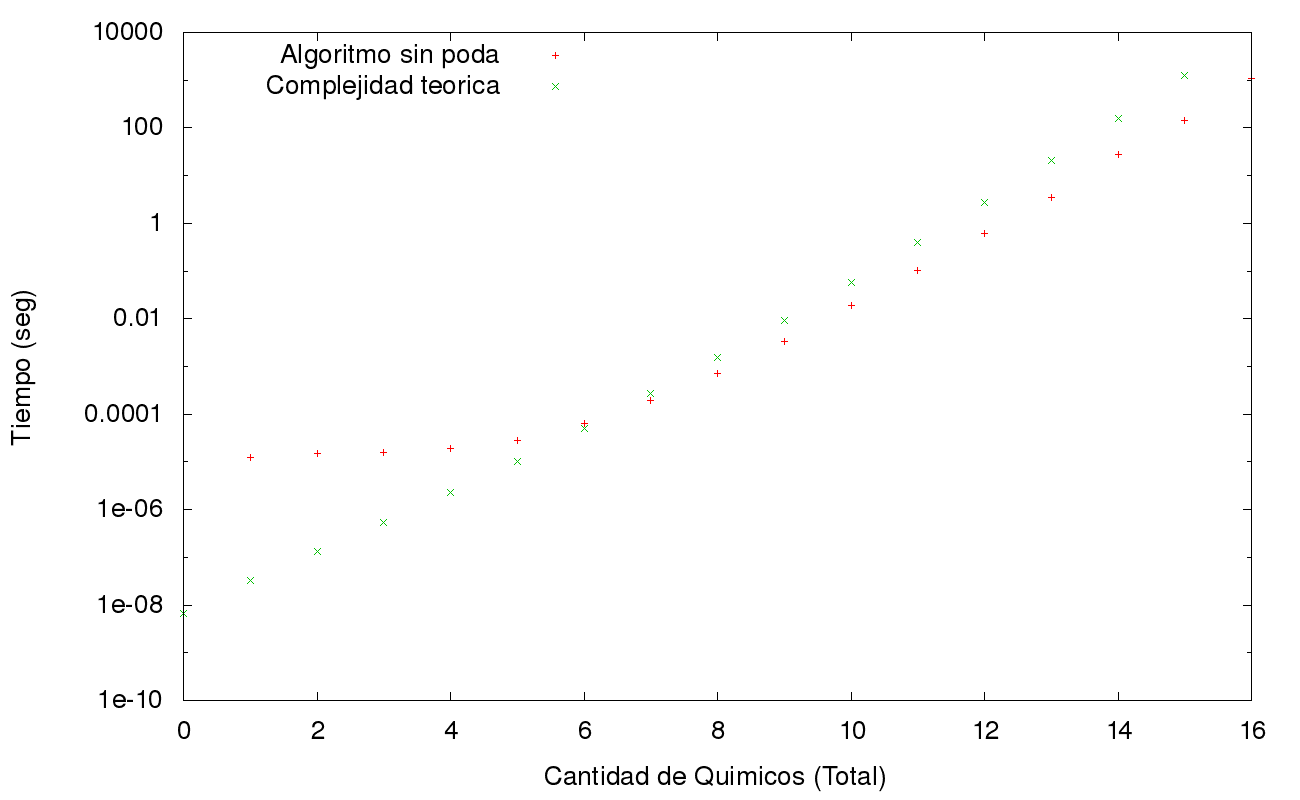
\includegraphics[scale=.30]{./imagenes/ej3_chartComplejidad.png}
\caption{Gr\'afico comparacion de rendimiento del Algoritmo con o sin poda.}
\end{center}
\end{figure}

\begin{figure}[H]
\begin{center}
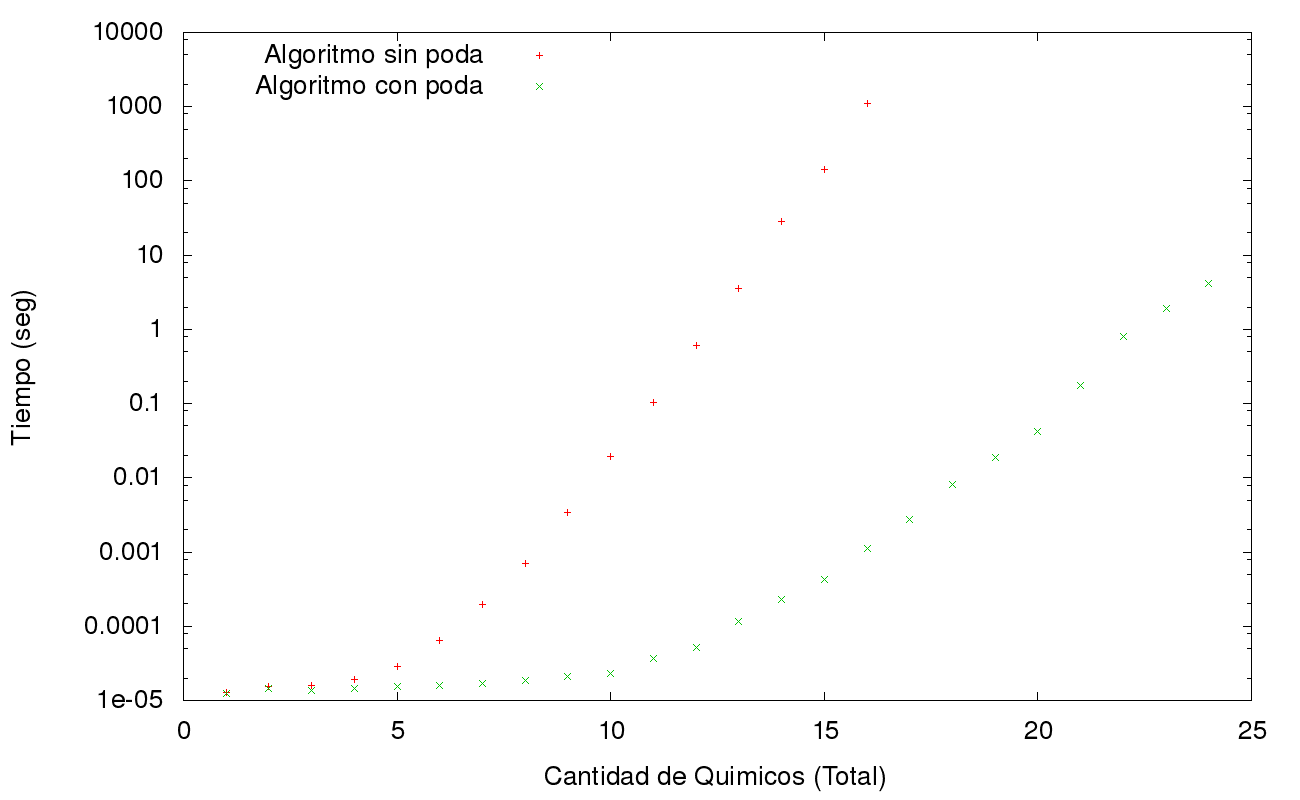
\includegraphics[scale=.30]{./imagenes/ej3_chartRendimiento.png}
\caption{Gr\'afico complejidad teorica vs practica.}
\end{center}
\end{figure}



\subsection{Extras}

\noindent 
La empresa est\'a a punto de contratar nuevos camiones y esta nueva flota no ser\'a homog\'enea, en el sentido del equipamiento de seguridad de los camiones. Con esto, cada cami\'on tendr\'a definido un umbral de peligrosidad distinto. Se pide desarrollar los siguientes puntos:

\noindent 
1. ¿C\'omo afecta eso a su algoritmo?

\noindent 
En primer lugar deber\'ia cambiar la entrada del algoritmo. Habr\'ia que agregar como entrada un n\'umero de peligrosidad por cada cami\'on disponible. Lo que llega a considerar lo siguiente: \\
Antes contabamos con todos los camiones que quisieramos, dado que ahora los camiones son algo que recibimos con una cantidad especificas, esto podr\'ia no seguir siendo as\'i. De todas maneras suponemos por el bien del problema y nuestra salud mental, dado que no est\'a especificado, que hay tantos camiones como qu\'imicos, de esta manera nunca me podr\'ia quedar sin camiones para ubicar alg\'un qu\'imico. \\
En segundo lugar el algoritmo que hicimos deber\'ia ser despedazado completamente. Dado que el umbral depende de cada cami\'on, est\'a mal considerar que no importa en qu\'e cami\'on va un set de qu\'imicos agrupado. En este caso, el cami\'on si importa. Se deber\'ia reemplazar el backtracking para que itere por cada quimico probando en todos los camiones. No s\'olo los camiones que ya tienen qu\'imicos, ni tampoco poniendo el qu\'imico en s\'olo el proximo cami\'on vac\'io. \\

\noindent 
2. ¿Qu\'e cosas se pod\'ıan hacer con el problema anterior para acelerar los tiempos de ejecuci\'on que ahora ya no se pueden? (es posible que la respuesta del item anterior responda esta pregunta).

\noindent 
S\'i, efectivamente creemos que de alguna manera respondimos esa pregunta. La primer poda es obsoleta. No se puede eliminar soluciones (con el nombre que nos referimos anteriormente en este informe) \textbf{practicamente iguales}. 

\subsection{Cambios}

Se refactorizó completamente el algoritmo que resolvía el problema. También se rehizo todo el parser. 
El informe está hecho de 0 con los nuevos cambios.


 


